\documentclass[12pt]{article}
\usepackage{fullpage,url,amssymb,epsfig,color,xspace,tikz,amsmath, amsthm}
\usetikzlibrary{matrix,backgrounds}

\begin{document}
    
\begin{center}
    \textbf{\huge Tutorial 5}
\end{center}

\section{Queue}
\begin{itemize}
    \item A queue is a container of data that enforces a \textbf{FIFO} policy on adds/removes
    \begin{itemize}
        \item e.g. order in Tim Hortons
    \end{itemize}
    \item Definition of stack: A stack is an ordered container of data that enforces 
            a \textbf{LIFO} policy on adds/removes
    \begin{itemize}
        \item e.g. back/forward button on browser
    \end{itemize}
    \item implementation of queue using vector(sapce inefficient)
    \item implementation of queue using linked list
\end{itemize}

\section{C++ arrays}
\begin{itemize}
    \item Static (as in C)
    \begin{itemize}
        \item Storage allocated on the stack
        \item Array bound (N) must be a compile-time constant
        i.e., it can be determined by just looking at the code and not running the program
    \end{itemize}
    \item C++ style dynamic arrays
    \begin{itemize}
        \item Storage is allocated on the heap via a call to new
        \item Array bound can be a run-time value (positive integer)
        \item Must delete when done, need to say "[ ]"!
    \end{itemize}

\end{itemize}

\section{Testing}
\begin{itemize}
    \item Black-box Testing
        \begin{itemize}
            \item Test a class/method against what it is supposed to do, but
            without looking at how the code achieves it
        \end{itemize}
    \item White-box Testing
        \begin{itemize}
            \item Try to exercise all parts of the underlying implementation
            \item Test against how the code is built, rather than what it is supposed to do
        \end{itemize}
\end{itemize}

 \section{exercises}
 \begin{enumerate}
    \item Implement queue using the struct below where 
    \begin{itemize}
        \item arr has fixed length "size"
        \item frt stores the index of first element
        \item last stores the index of last element
        \item the next element of arr[size - 1] is arr[0]
    \end{itemize}
    \begin{verbatim}
struct Queue {
  int size;
  int frt;
  int last;
  int *arr;
};
void init(Queue &q, int size);
//if queue is full, replace the oldest element in the queue
void add(Queue &q, int val);
void remove(Queue &q);
void print(Queue &q);
    \end{verbatim}    
    For example,\\
    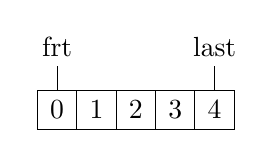
\begin{tikzpicture}[
        array/.style={matrix of nodes,nodes={draw, minimum size=7mm},column sep=-\pgflinewidth, row sep=0.5mm, nodes in empty cells,
        row 1/.style={nodes={minimum size=5mm}}}]
        \matrix[array] (array) {
        0 & 1 & 2 & 3 & 4 \\};
        \draw (array-1-1.north)--++(90:3mm) node [above] (first) {frt};
        \draw (array-1-5.north)--++(90:3mm) node [above] (first) {last};
    \end{tikzpicture}\\
    add(q, 6)\\
    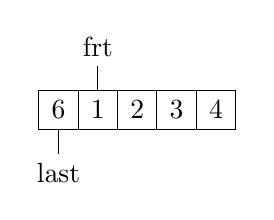
\begin{tikzpicture}[
        array/.style={matrix of nodes,nodes={draw, minimum size=7mm},column sep=-\pgflinewidth, row sep=0.5mm, nodes in empty cells,
        row 1/.style={nodes={minimum size=5mm}}}]
        \matrix[array] (array) {
        6 & 1 & 2 & 3 & 4 \\};
        \draw (array-1-2.north)--++(90:3mm) node [above] (first) {frt};
        \draw (array-1-1.south)--++(-90:3mm) node [below] (first) {last};
    \end{tikzpicture}
    
    \newpage \item Write test cases for the following Queue operations:
    \begin{itemize}
        \item enqueue
        \item dequeue
        \item containsElement
        \item isEmpty
    \end{itemize}
    \begin{verbatim}
#include <iostream>
#include <string>
#include <vector>

using namespace std;


typedef vector<string> Queue;


void enqueue(Queue q, string data);
void dequeue(Queue& q);
bool isEmpty(Queue& q);
bool containsElement(Queue& q, string s);

int main() {
	// Put your tests here
}

bool isEmpty(Queue& q) {
	return q.empty();
}

void enqueue(Queue q, string data) {
	q.push_back(data);
}

void dequeue(Queue& q) {
	if(!isEmpty(q)) {
		q.pop_back();
	}
}

bool containsElement(Queue& q, string s) {
		
	for(string next : q) {
		return next == s;
	}
	
	return false;
	
}
    \end{verbatim}
 \end{enumerate}

\end{document}